\section{Evaluation}\label{s:eval}

\FYI{

# Ext4
-
- Score

# F2FS
- Score

# Fragmentation on FDP?
}


\begin{comment}
초반 - 실험 환경 설명 Eval Setup

들어가야 하는 내용 :
  1. 실제로 노화가 영향을 주나? => latency과 dynamic score를 비교하며, dynamic score과 반비례하여 latency가 증가한다.
								 왜 이런 결과가 나오는지? fragmentation 때문인데, 이걸 그림과 대조하며 설명.
								 근데 어떤 그림을 사용해야 할지 고민됨.

  2. dump하는데 필요한 저장공간 => 그래서 update된 storage부분만 snapshot뜨기로 함. => 이건 어느정도?
 	 전체 storage를 dump vs update된 storage만 dump 했을 때의 시간 차이
	 => 큰 차이는 없고 데이터 배치에 따라 결과값이 달라짐.
	 => 굳이 따지면 save는 update된 storage만 dump하는게 조금떠 빠르고 load는 느리게 관측됨
	 => 왜지..?


\end{comment}



We evaluated using several workloads to aging the stroage system.
%  Git workload
The Git aging benchmark\cite{conway:login17,senescence:fast17} can incur aging in a real-world environment that people commonly use.
Git is a distributed version control system that allows synchronization of source code changes.
This benchmark generates workloads by simulating developers working on collaborative projects using Git.
Experiments are conducted using the git pull command, which creates new source files, deletes old files, or modifies files. During this process, Git maintains its internal data structure, leading to filesystem aging.
To measure the extent of aging, multiple git pull commands can be executed, and latency can be measured through reads using grep.

% ext4 workload

% f2fs workload

% rocksdb workload

% what is dynamic score


% Setup
\subsection{Evaluation Environment}
\begin{comment}
=> NVMEVIRT를 사용한 가상환경에서 실험을 진행함.
=> 컴퓨터의 스펙은 동일하게(mir1의 cpu, mem, storage를 설명), nvmevirt는 conv로, storage의 크기만 다르게 해서 실험을 진행함.
=> nvmevirt가 구현된 커널 스펙
=> Line of code
\end{comment}
I need to Write..

% Aging affects the performance of storage

% comparison snapshot latency
\subsection{Comparison snapshot Latency}
[] dumps the storage.
Therefore, if the original contents of a 1TB storage are copied, a 1TB snapshot is created.
However, not all parts of the storage contain data.
[] only dumps the portions of the storage where meaningful data is stored.

\begin{figure}[t]
    \centering
	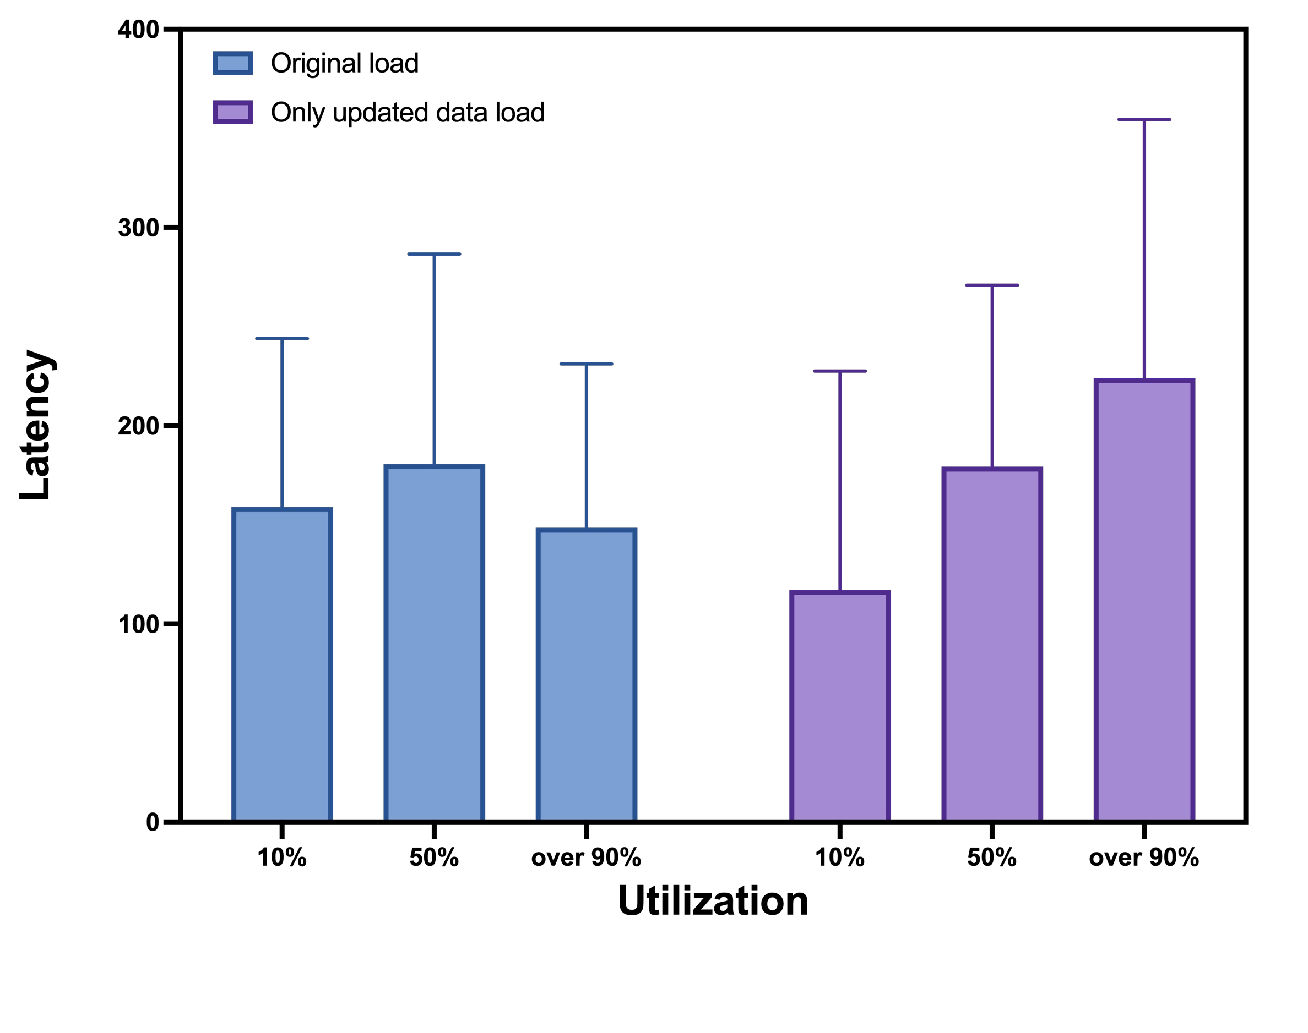
\includegraphics[width=0.95\columnwidth]{graphs/load_latency}
	\caption{Load Latency}
	\label{f:load_latency}
\end{figure}

\begin{figure}[t]
    \centering
	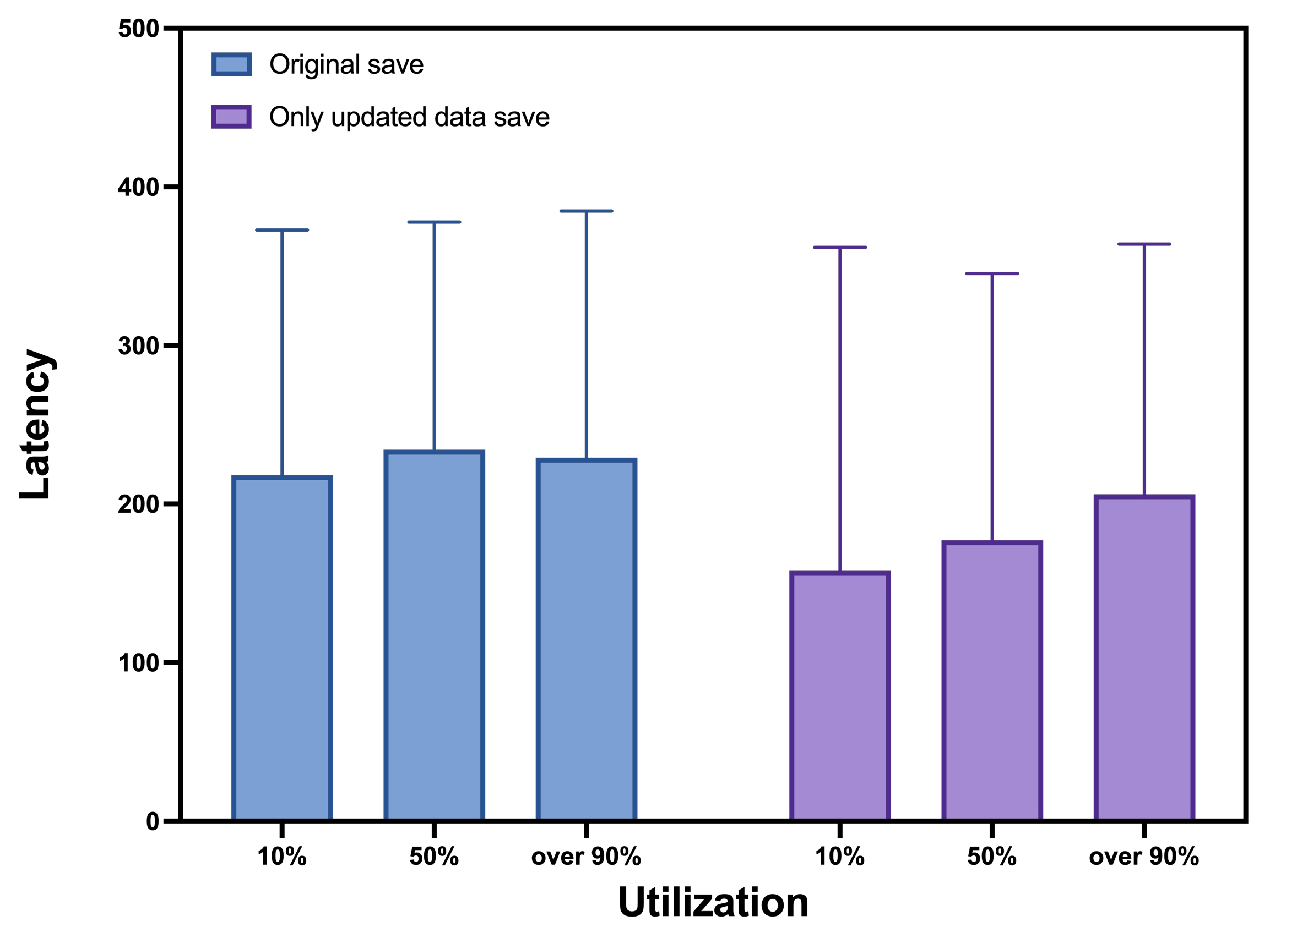
\includegraphics[width=0.95\columnwidth]{graphs/save_latency}
	\caption{Save Latency}
	\label{f:save_latency}
\end{figure}

Figures~\ref{f:save_latency} and \ref{f:load_latency} consider two scenarios: one where the entire storage is dumped and loaded, and another where only the updated data is dumped and loaded.
The results for each scenario, measured at storage utilization levels of 10\%, 50\%, and over 90\%, are presented in bar graphs for storage sizes of 16GB, 64GB, and 128GB.
The thick bars represent the average latency, while the thin lines indicate the maximum values.
A lower position of the lines and bars indicates shorter latency.

When comparing the two scenarios, the case of dumping only the updated data shows slightly lower latency.
However, in the loading scenario, higher latency is observed. This phenomenon arises from the loading method.
To load the updated data, it must be stored at specified addresses in the storage according to the information in the snapshot data.
At this point, the number of load calls can vary depending on the distribution of existing data.
For this reason, there may even be cases where the loading latency is lower.

In the case of saving, similar to loading, the number of save calls varies according to the distribution of stored data.
However, due to caching, the number of save commands reaching the storage device is lower compared to loading.

As shown in the graphs, these differences are not significant.
While dumping the entire storage is more stable in terms of latency, the scenario of dumping only the updated data does not show a large difference in latency.
Rather, the ability to work with a smaller snapshot size presents a greater advantage.


\begin{figure}[t]
    \centering
    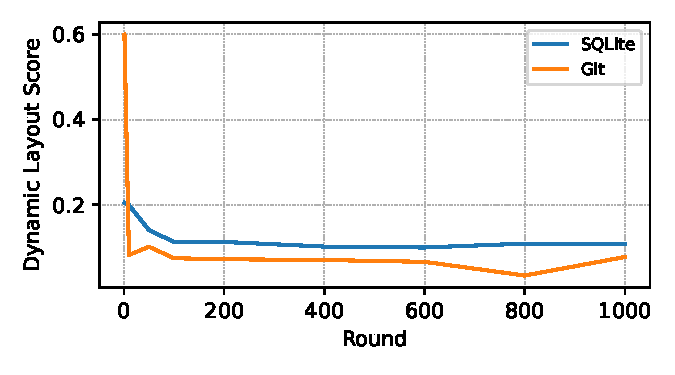
\includegraphics[width=0.95\columnwidth]{graphs/py_graph/dynamic}
    \caption{}
    \label{f:dynamic}
\end{figure}

\begin{figure}[t]
    \centering
    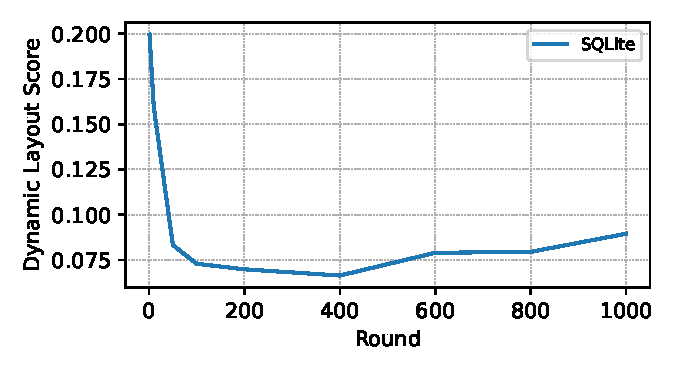
\includegraphics[width=0.95\columnwidth]{graphs/py_graph/dynamic-f2fs}
    \caption{}
    \label{f:f2fs_dynamic_score}
\end{figure}


\begin{figure}[t]
    \centering
    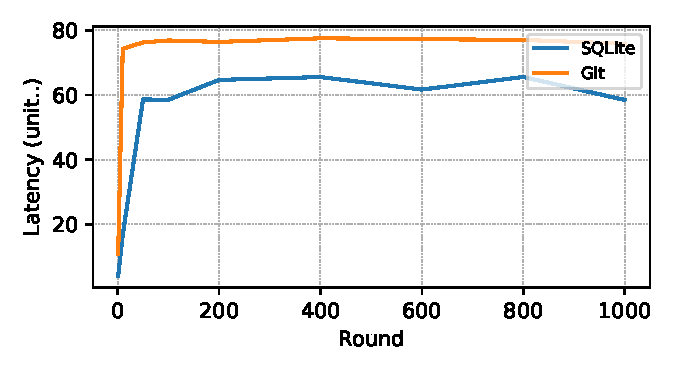
\includegraphics[width=0.95\columnwidth]{graphs/py_graph/latency}
    \caption{}
    \label{f:latency}
\end{figure}

\begin{figure}[t]
    \centering
    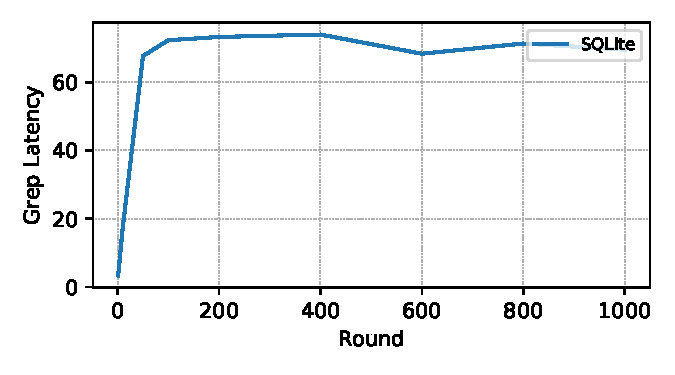
\includegraphics[width=0.95\columnwidth]{graphs/py_graph/latency-f2fs}
    \caption{}
    \label{f:f2fs_latency}
\end{figure}


\begin{figure}[t]
    \centering
	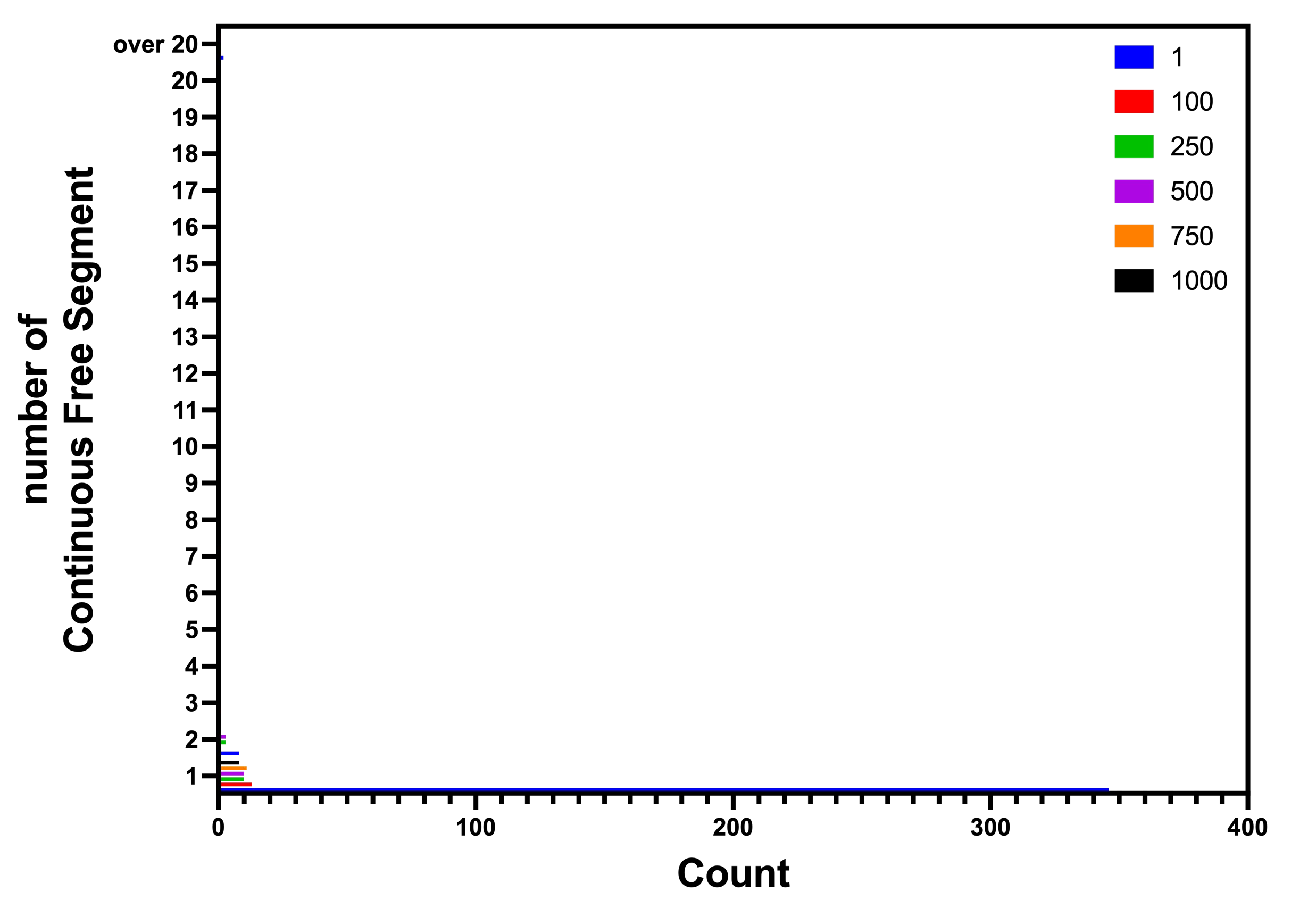
\includegraphics[width=0.95\columnwidth]{graphs/continuous_free_segment_fsfs}
	\caption{Continuous Free Segment-F2FS}
	\label{f:continuous_free_segment_fsfs}
\end{figure}

\begin{figure}[t]
    \centering
	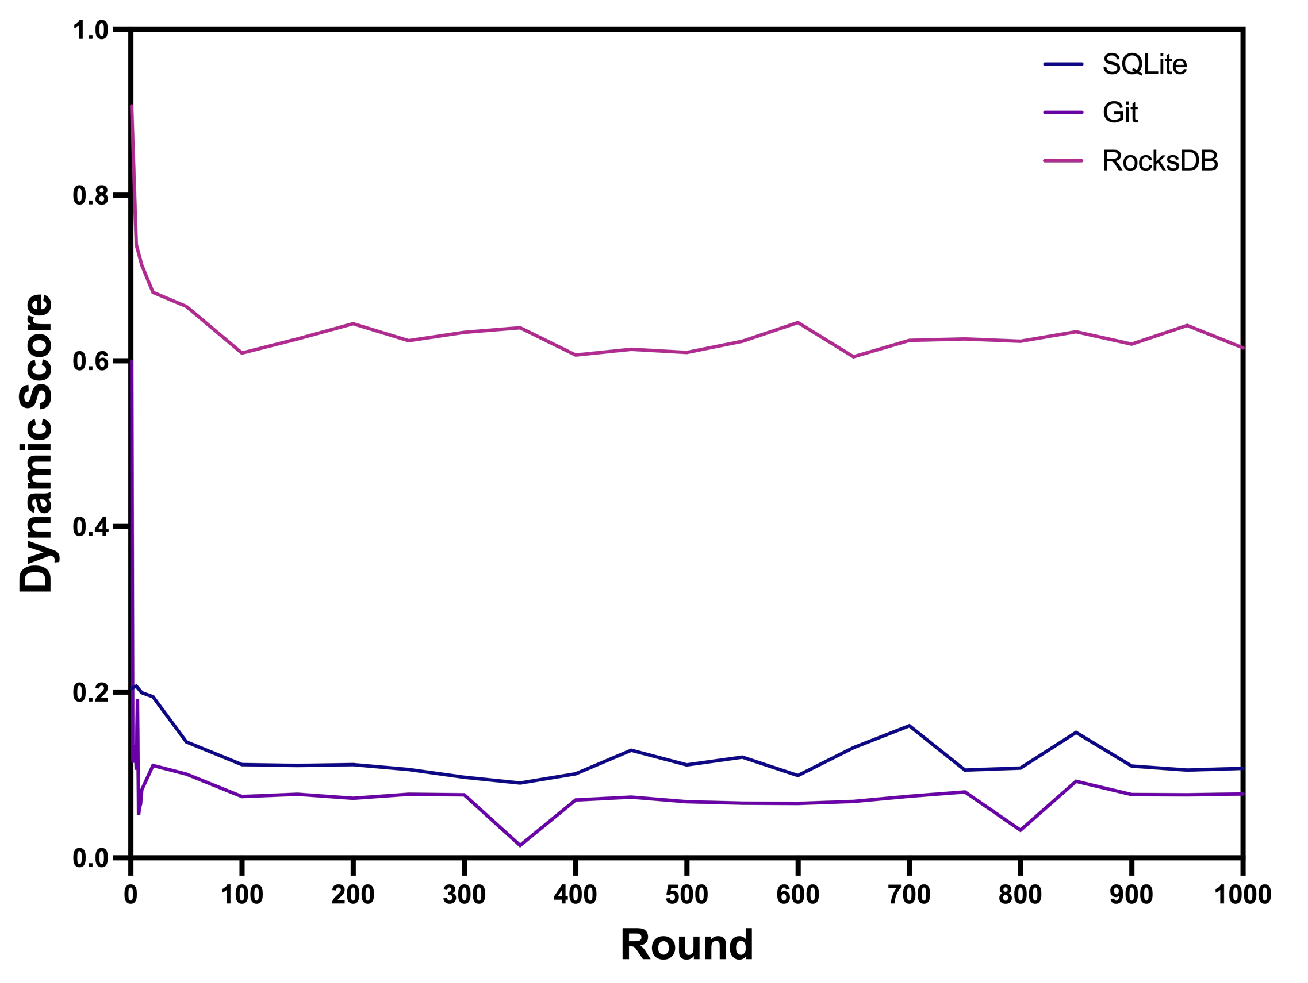
\includegraphics[width=0.95\columnwidth]{graphs/ext4_dynamic}
	\caption{Dynamic Score-EXT4}
	\label{f:ext4_dynamic}
\end{figure}


\begin{figure}[t]
    \centering
	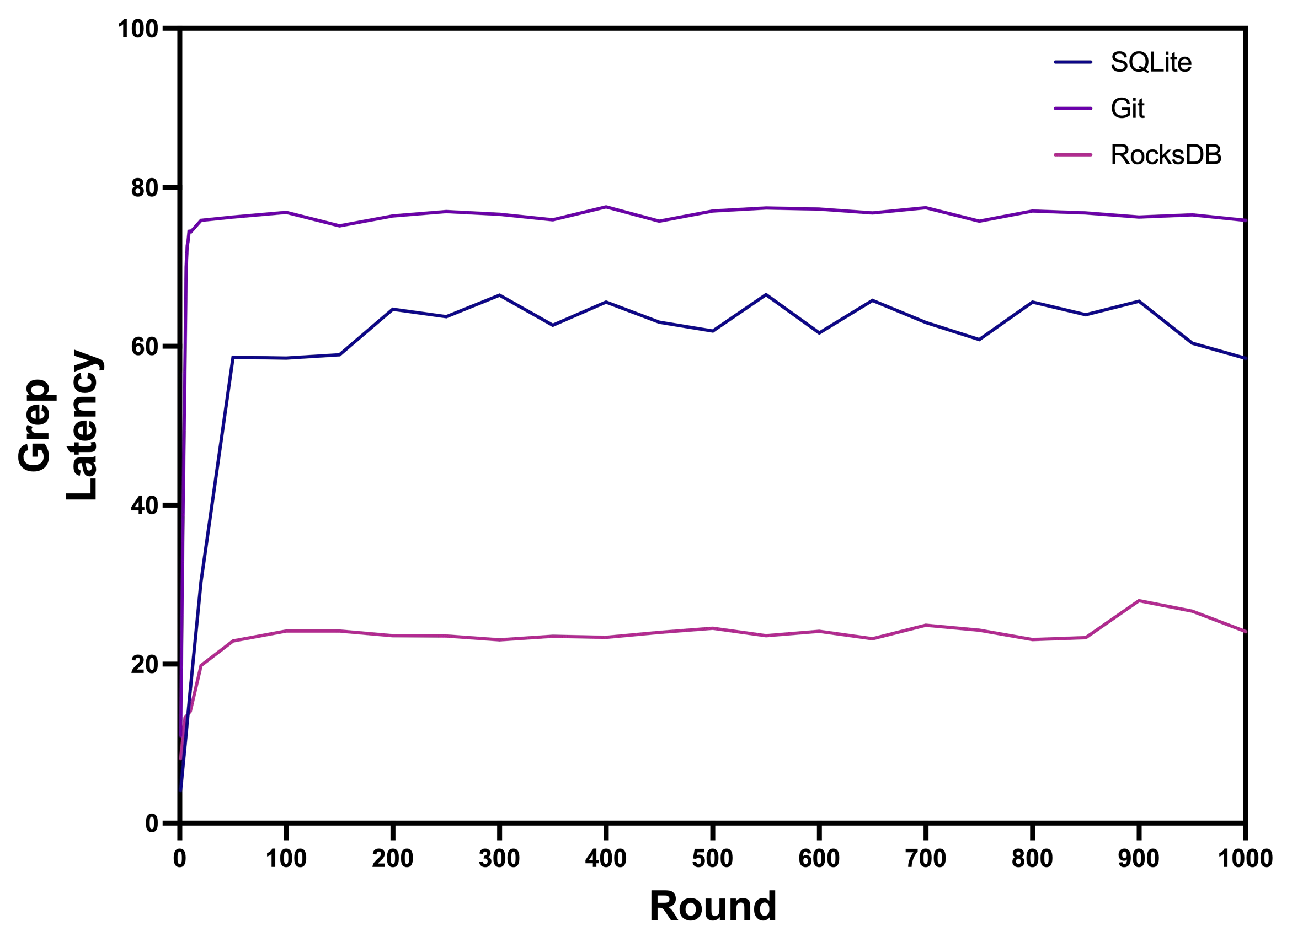
\includegraphics[width=0.95\columnwidth]{graphs/ext_latency}
	\caption{Latency-EXT4}
	\label{f:ext_latency}
\end{figure}

\begin{figure}[t]
    \centering
	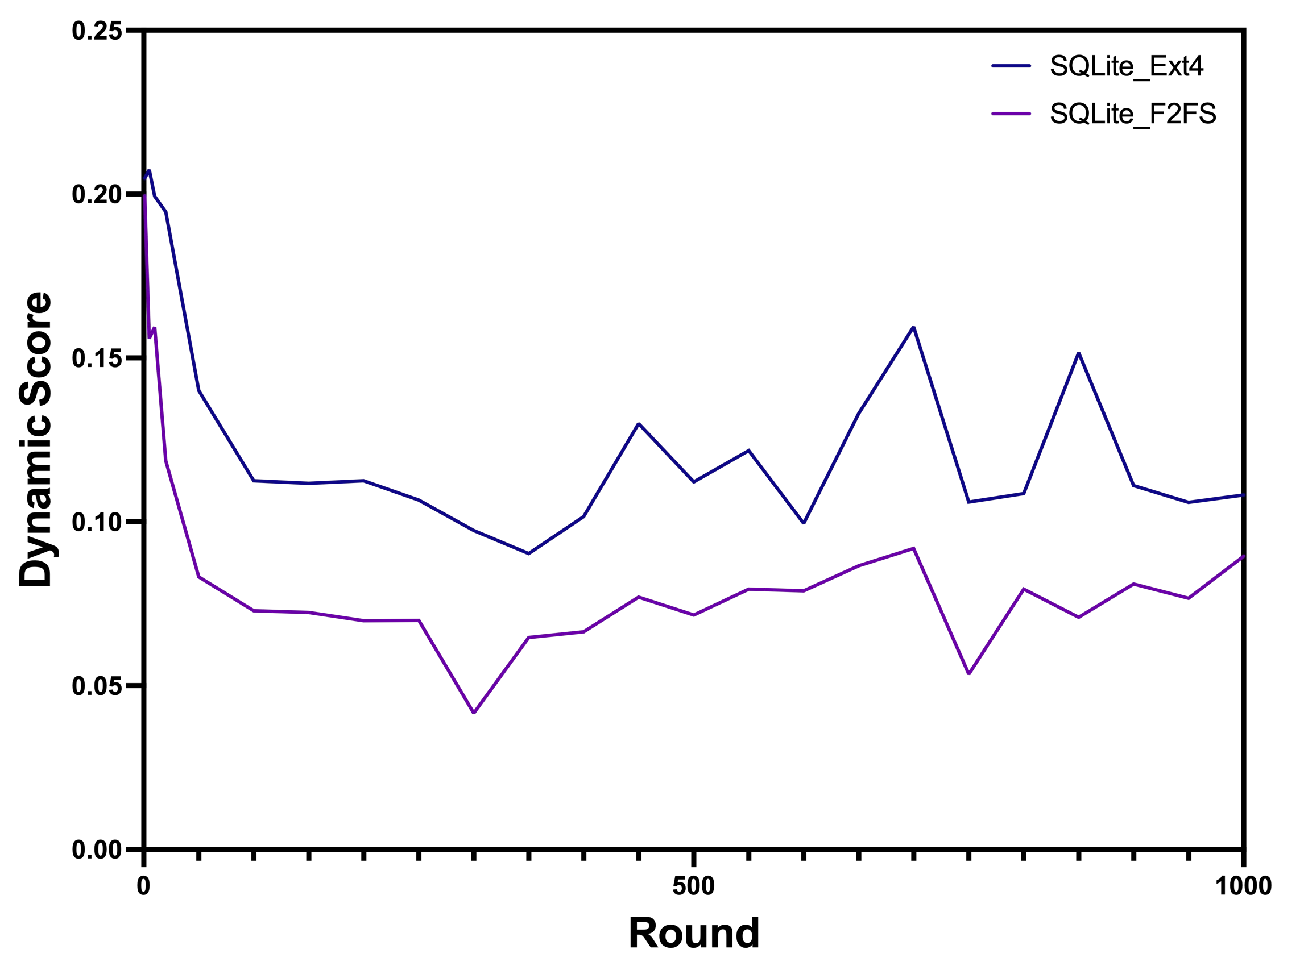
\includegraphics[width=0.95\columnwidth]{graphs/f2fs_vs_ext4_dynamic}
	\caption{Dynamic Score-F2FS vs EXT4}
	\label{f:f2fs_vs_ext4_dynamic}
\end{figure}


\begin{figure}[t]
    \centering
	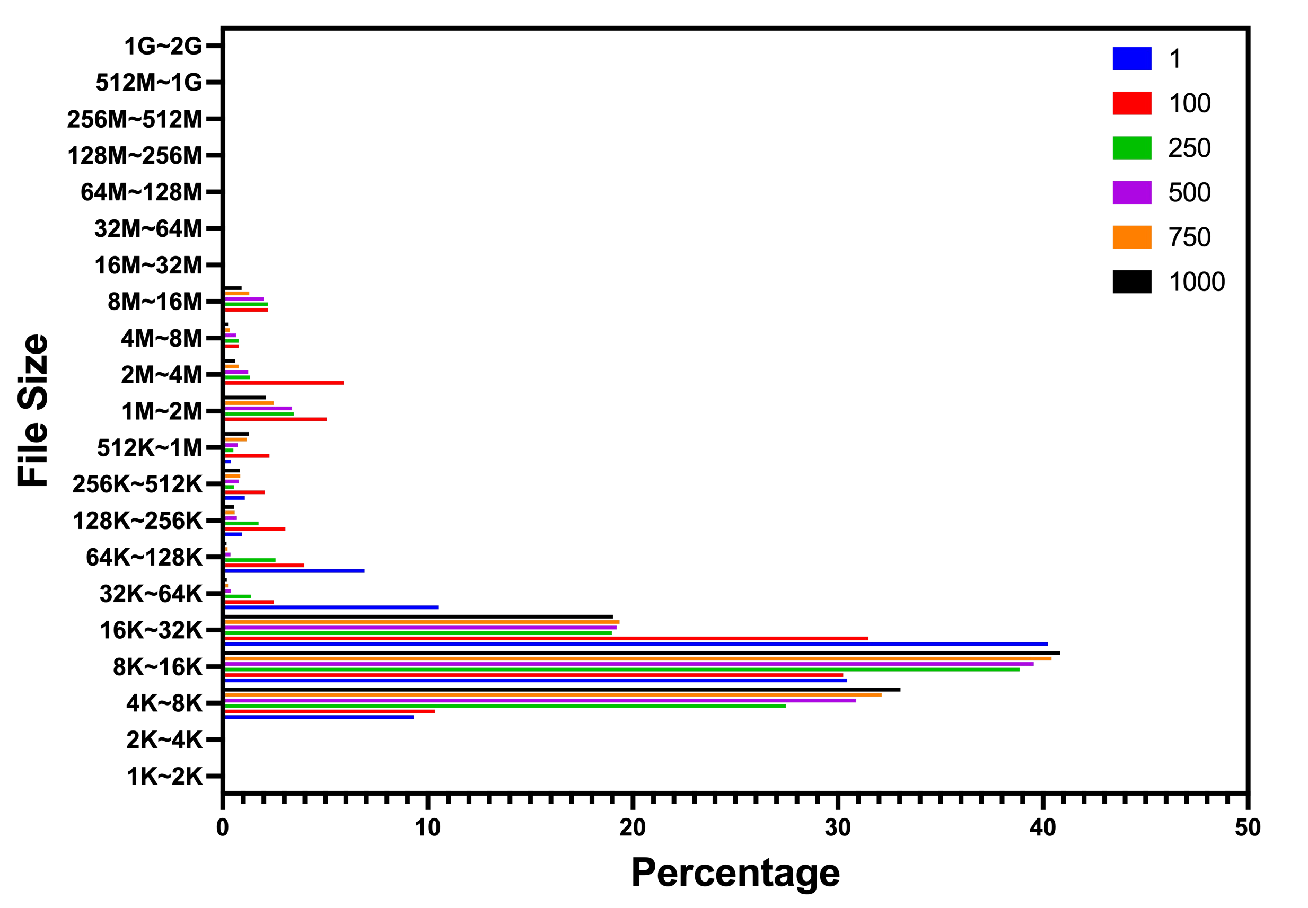
\includegraphics[width=0.95\columnwidth]{graphs/file_block_ext4}
	\caption{File Block-EXT4}
	\label{f:file_block_ext4}
\end{figure}

\begin{figure}[t]
    \centering
	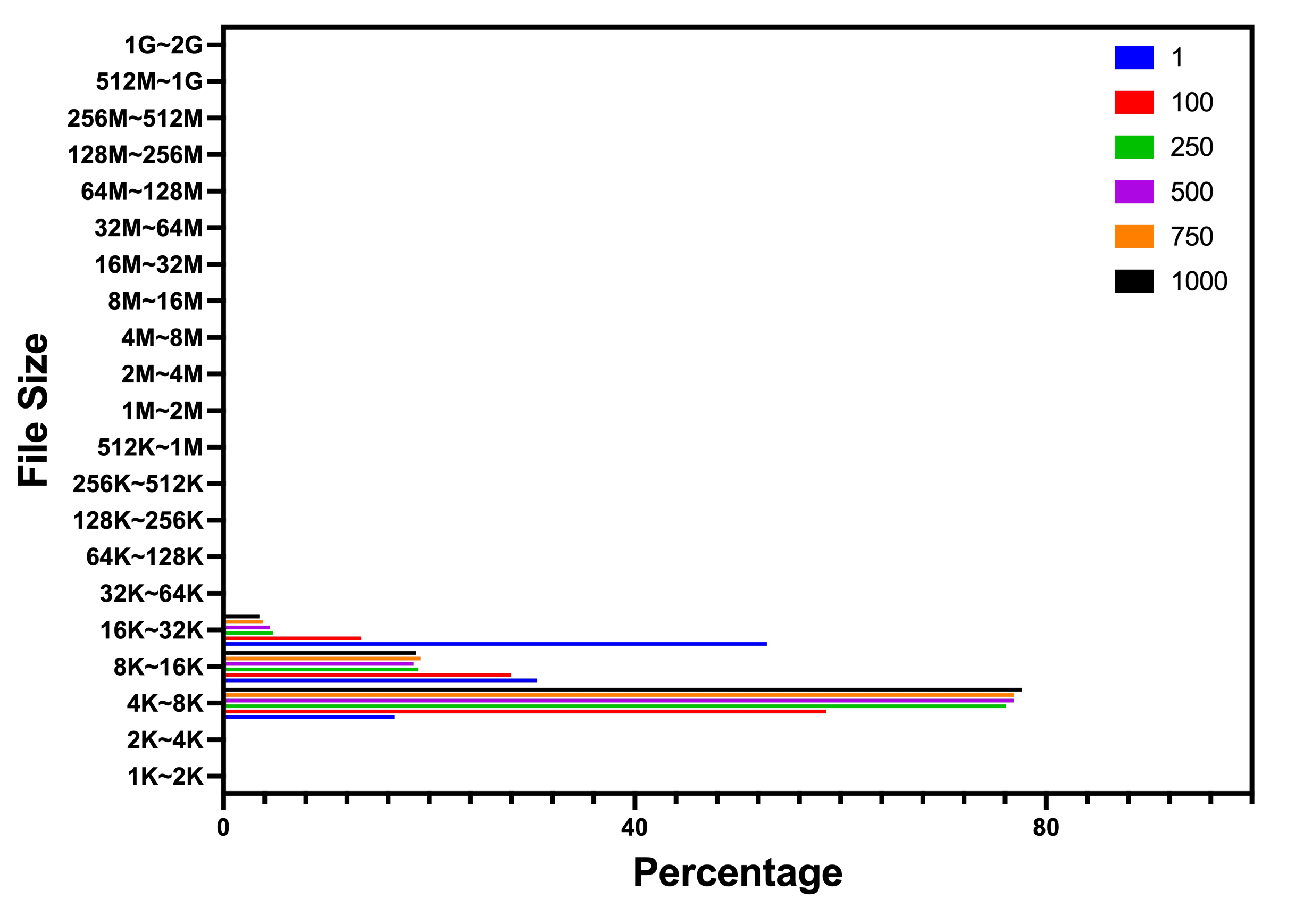
\includegraphics[width=0.95\columnwidth]{graphs/file_block_f2fs}
	\caption{File Block-F2FS}
	\label{f:file_block_f2fs}
\end{figure}

\begin{figure}[t]
    \centering
	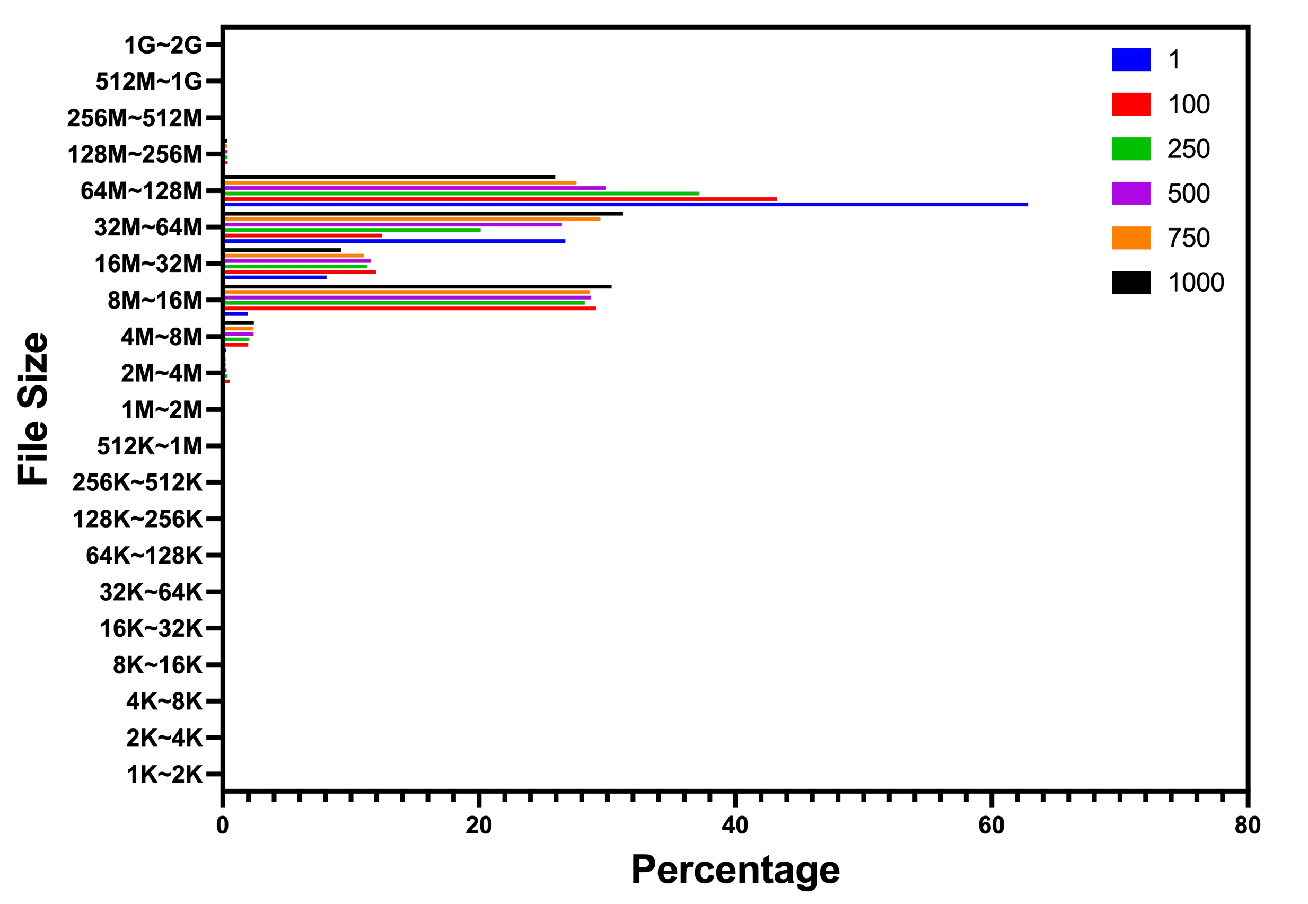
\includegraphics[width=0.95\columnwidth]{graphs/file_block_rocksdb}
	\caption{File Block-RockDB}
	\label{f:file_block_rocksdb}
\end{figure}

\begin{figure}[t]
    \centering
	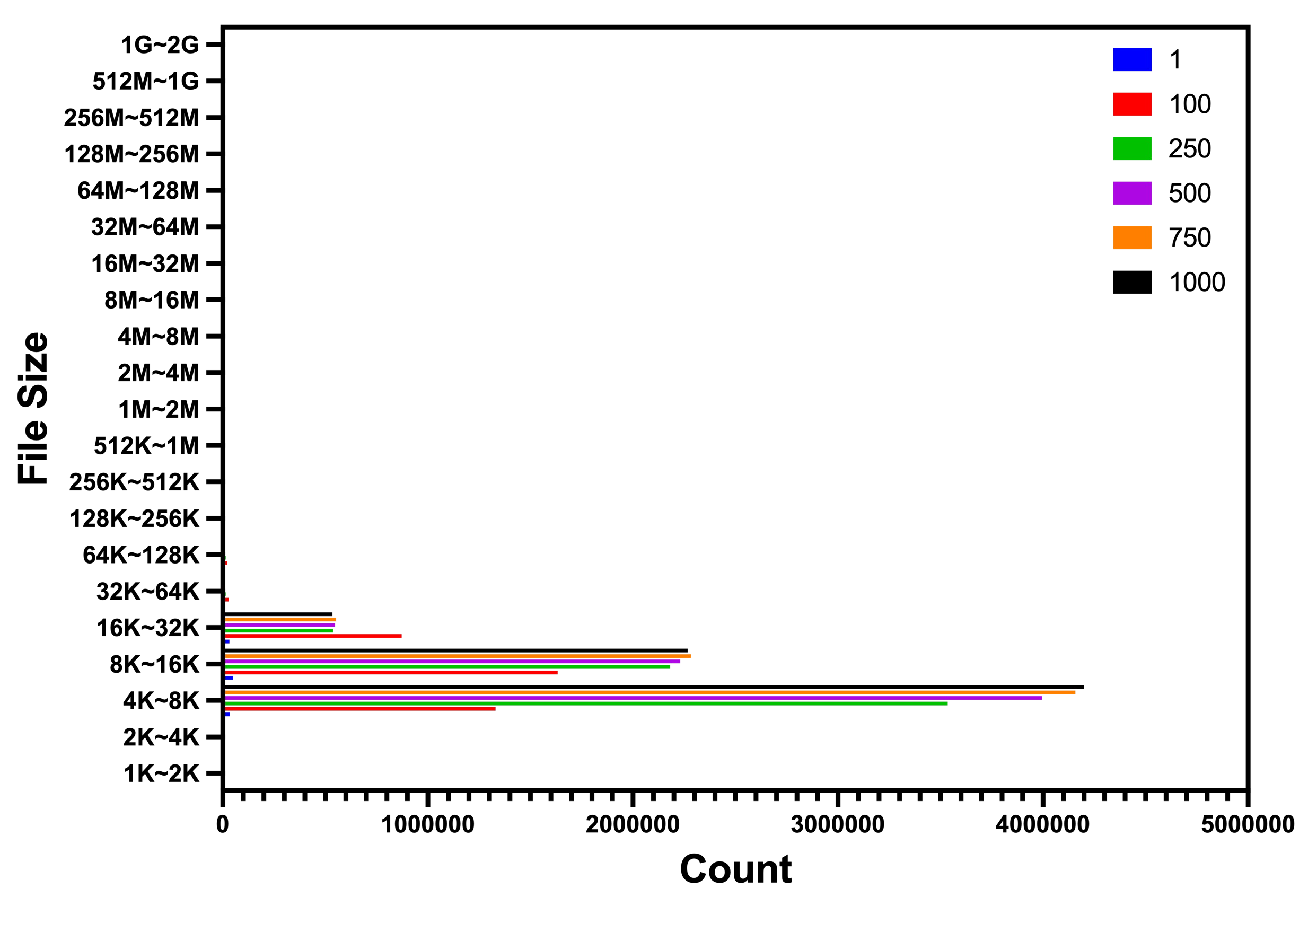
\includegraphics[width=0.95\columnwidth]{graphs/file_extents_ext4}
	\caption{File Extents-EXT4}
	\label{f:file_extents_ext4}
\end{figure}

\begin{figure}[t]
    \centering
	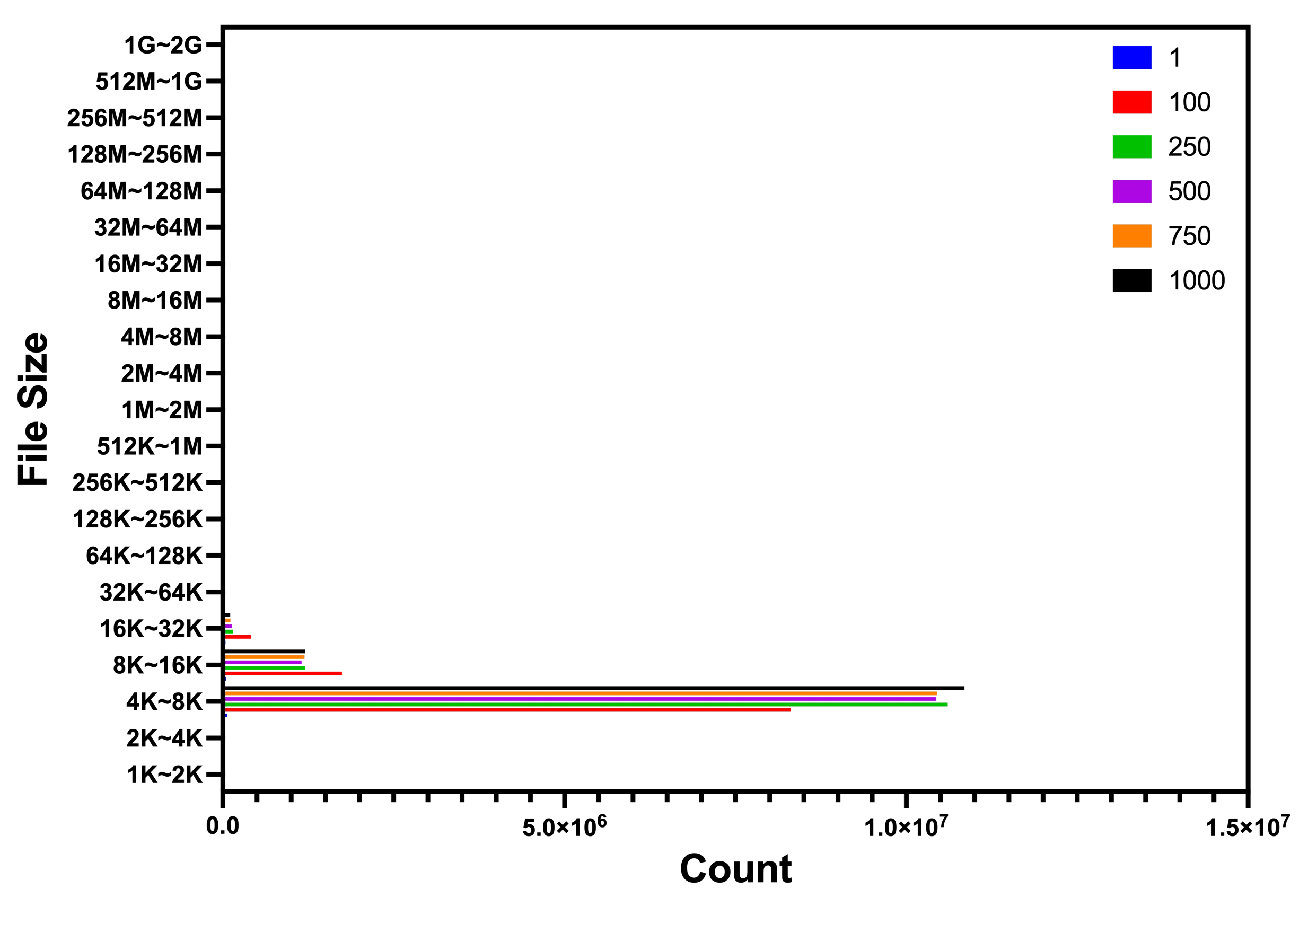
\includegraphics[width=0.95\columnwidth]{graphs/file_extents_f2fs}
	\caption{File Extents-F2FS}
	\label{f:file_extents_f2fs}
\end{figure}

\begin{figure}[t]
    \centering
	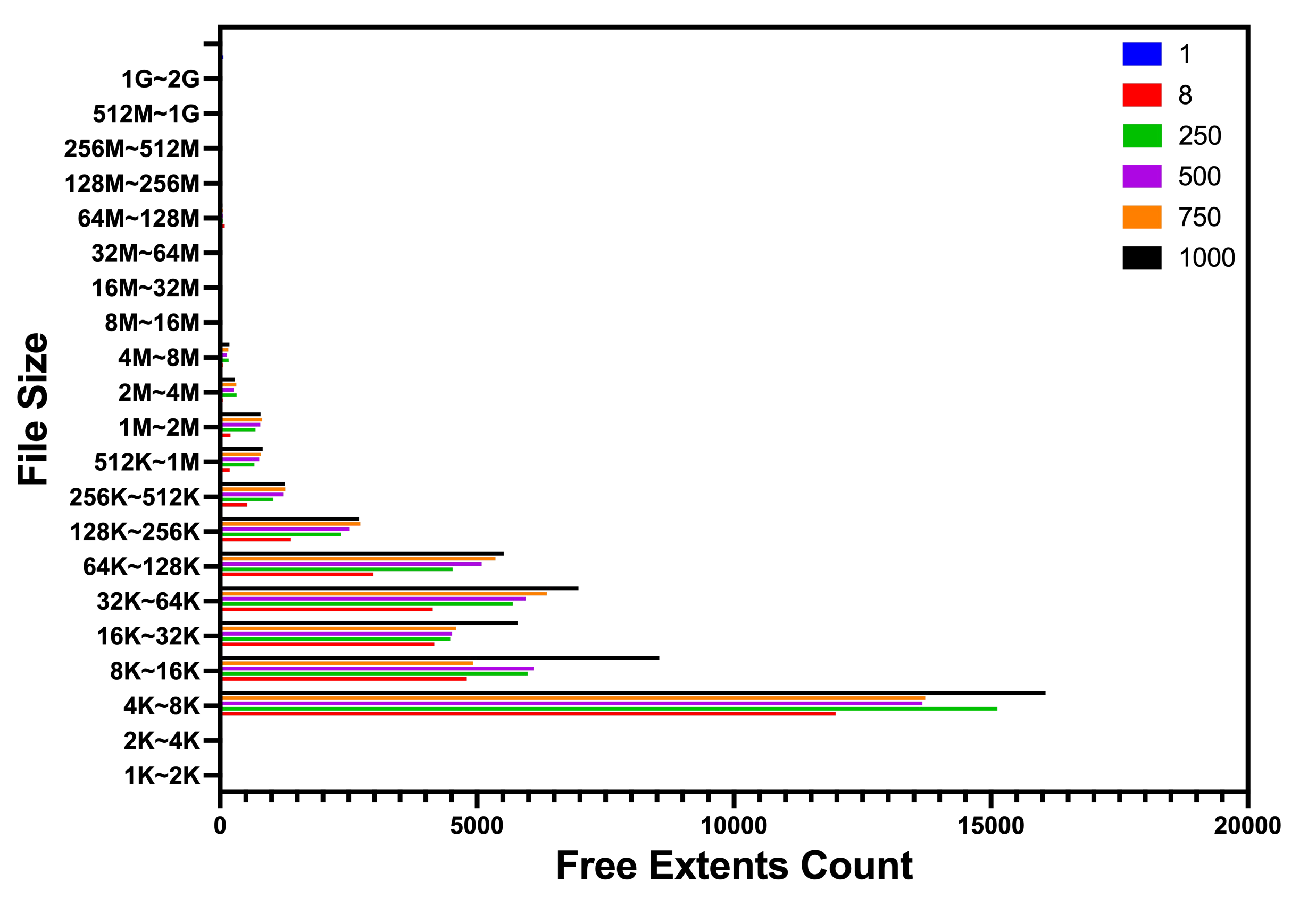
\includegraphics[width=0.95\columnwidth]{graphs/file_extents_git}
	\caption{File Extents-GIT}
	\label{f:file_extents_git}
\end{figure}

\begin{figure}[t]
    \centering
	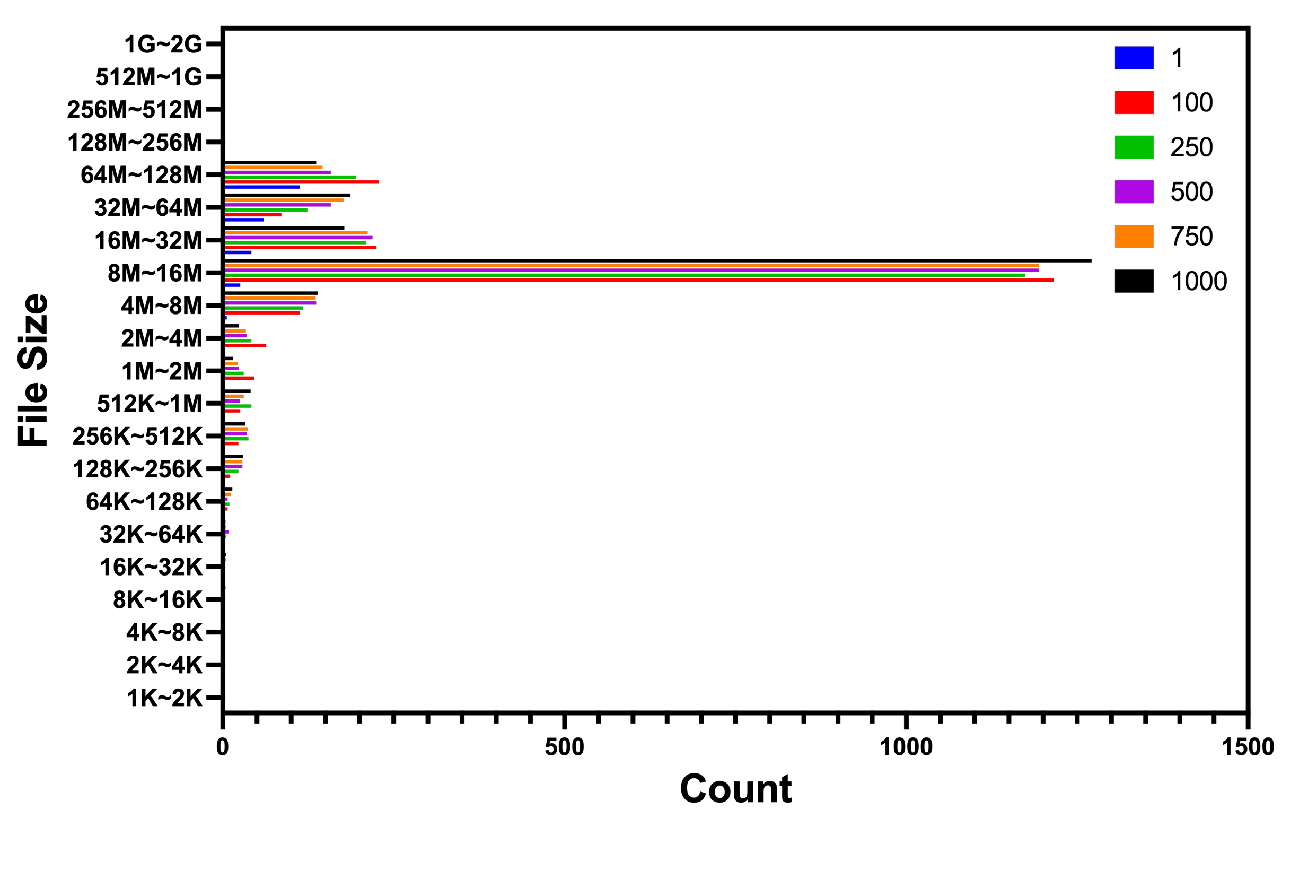
\includegraphics[width=0.95\columnwidth]{graphs/file_extents_rocksdb}
	\caption{File Extents-RocksDB}
	\label{f:file_extents_rocksdb}
\end{figure}

\begin{figure}[t]
    \centering
	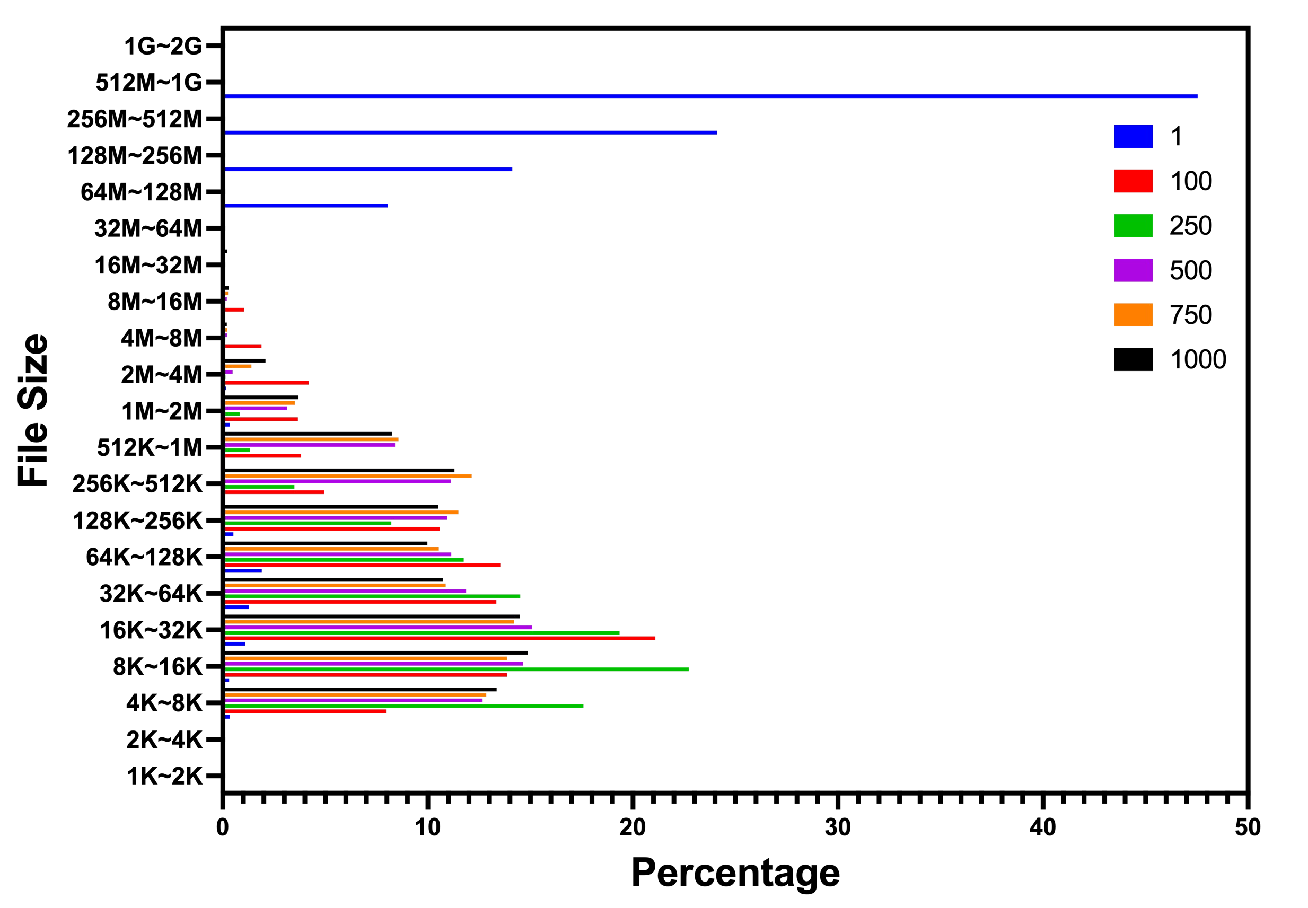
\includegraphics[width=0.95\columnwidth]{graphs/free_block_ext4}
	\caption{Free Block-EXT4}
	\label{f:free_block_ext4}
\end{figure}

\begin{figure}[t]
    \centering
	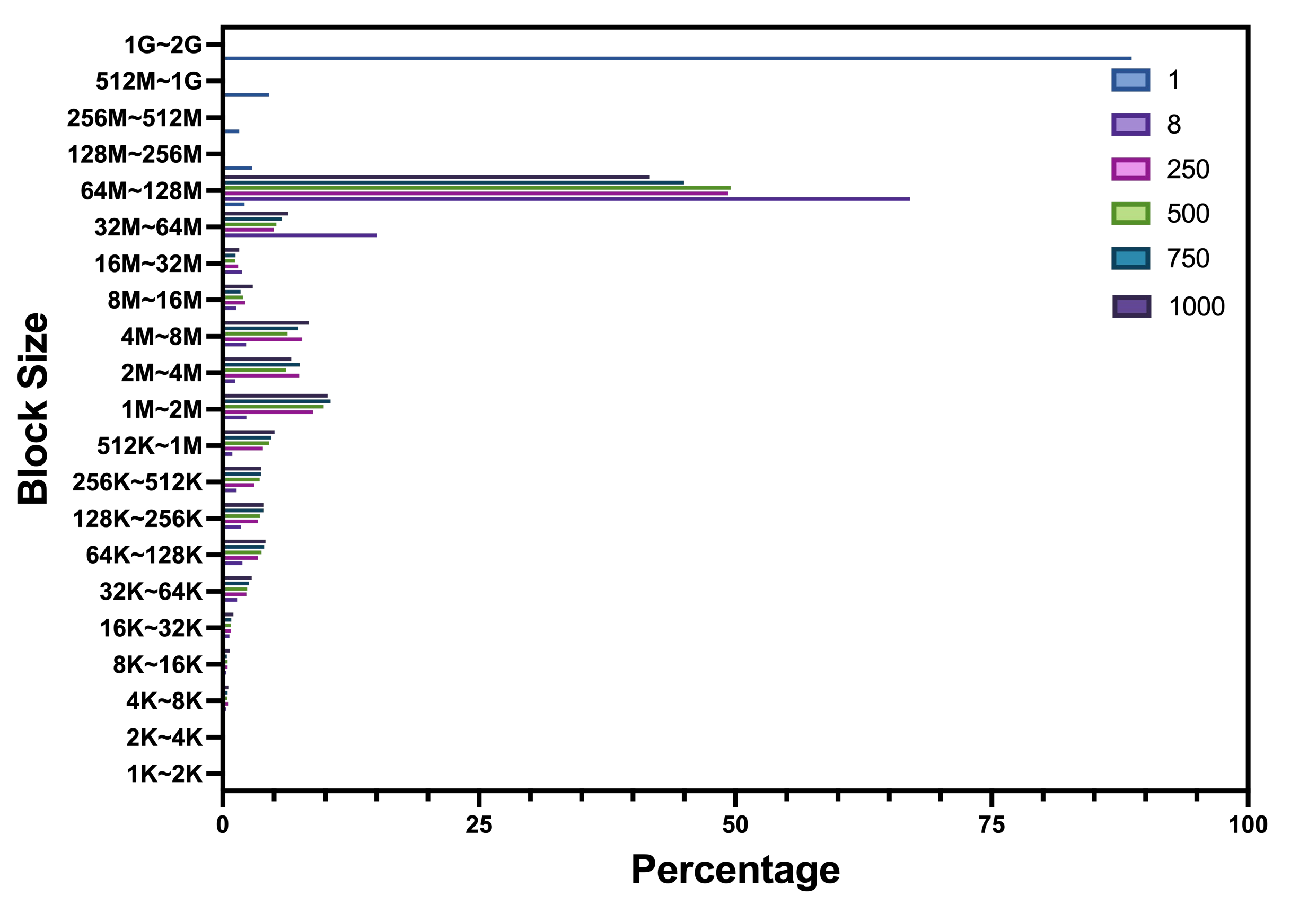
\includegraphics[width=0.95\columnwidth]{graphs/free_block_git}
	\caption{Free Block-GIT}
	\label{f:free_block_git}
\end{figure}

\begin{figure}[t]
    \centering
	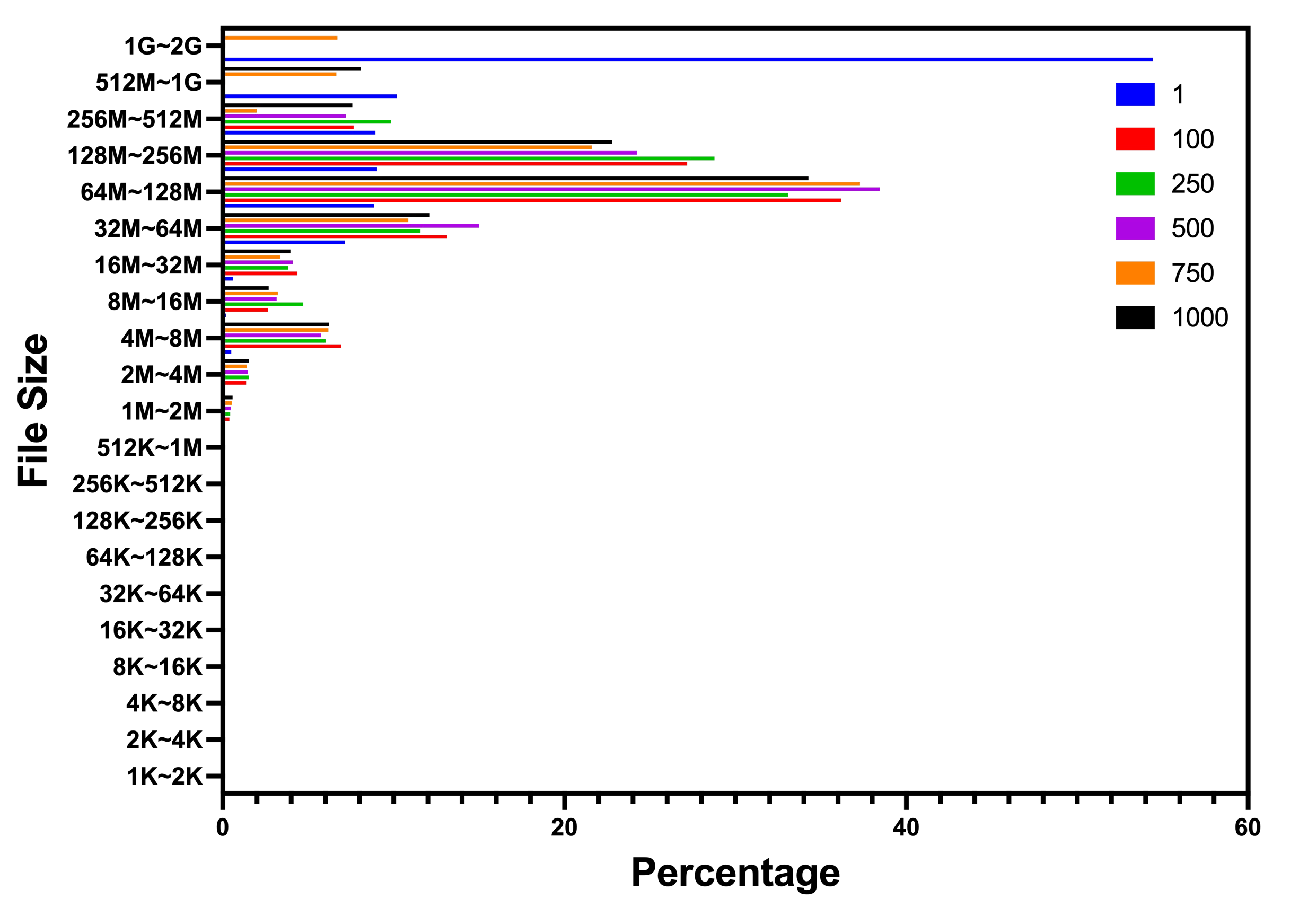
\includegraphics[width=0.95\columnwidth]{graphs/free_block_rocksdb}
	\caption{Free Block-RockDB}
	\label{f:free_block_rocksdb}
\end{figure}

\begin{figure}[t]
    \centering
	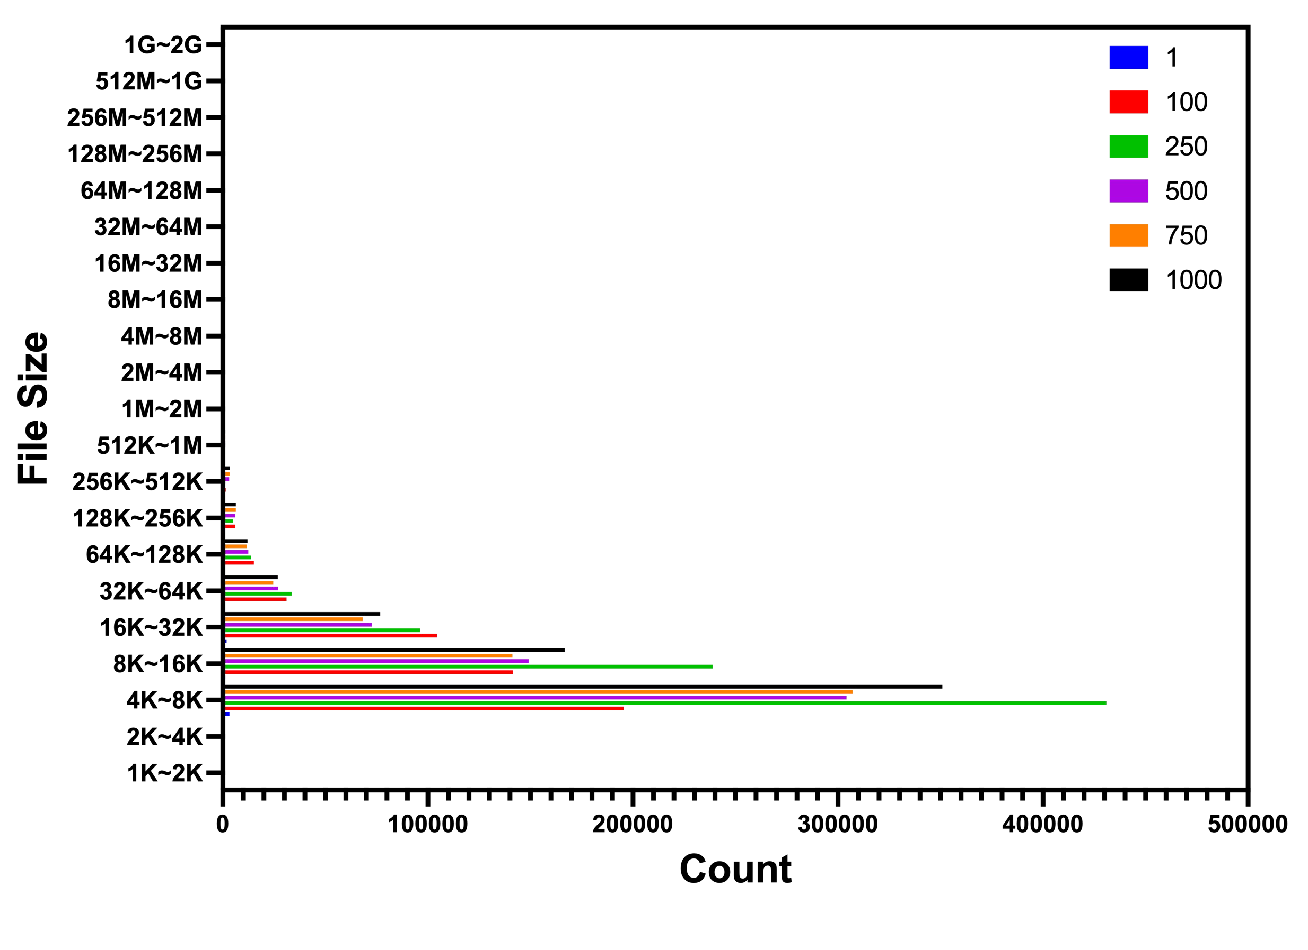
\includegraphics[width=0.95\columnwidth]{graphs/free_extents_ext4}
	\caption{Free Extents-EXT4}
	\label{f:free_extents_ext4}
\end{figure}

\begin{figure}[t]
    \centering
	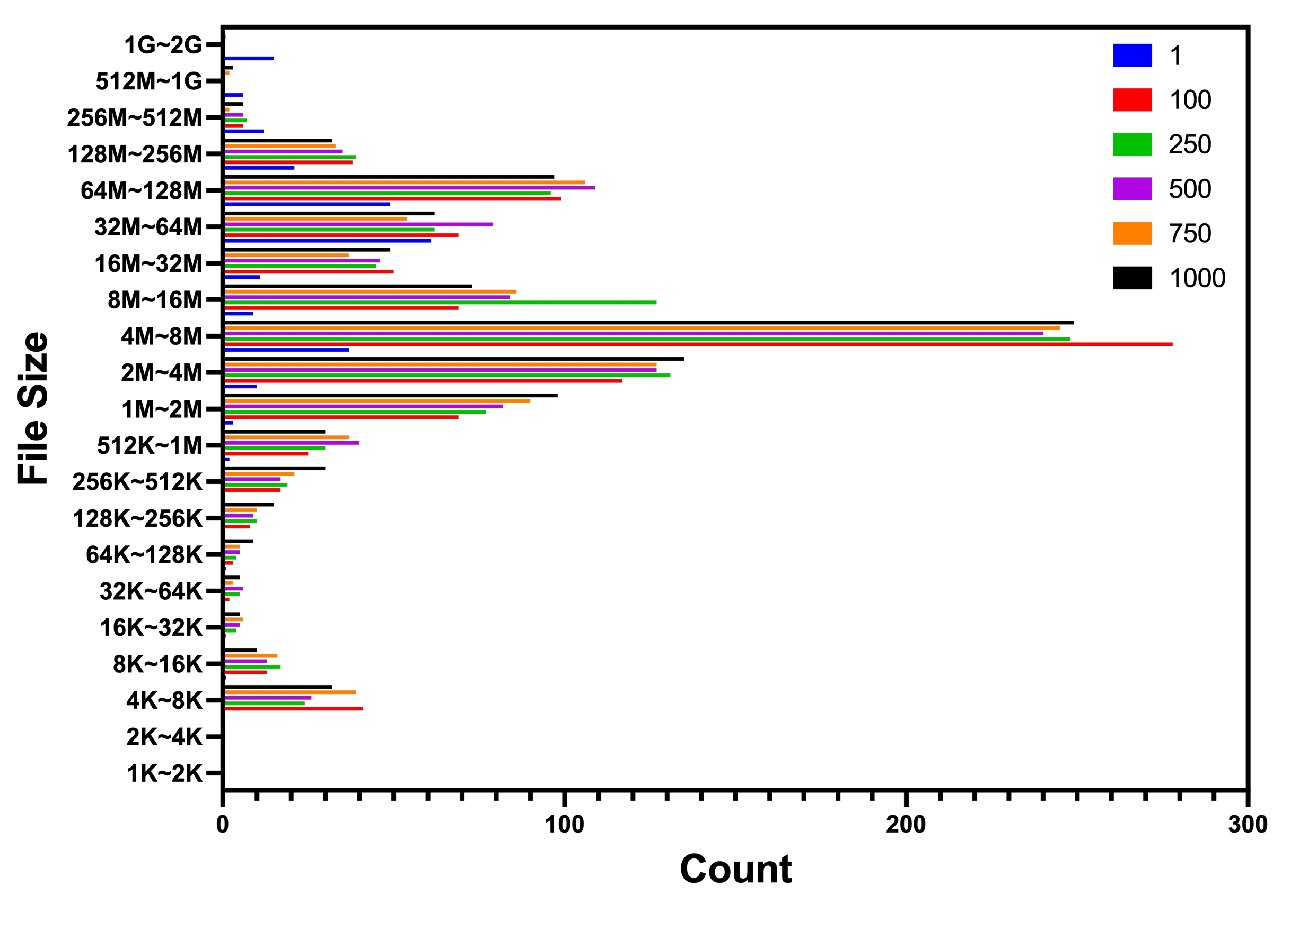
\includegraphics[width=0.95\columnwidth]{graphs/free_extents_rocksdb}
	\caption{Free Extents-RockDB}
	\label{f:free_extents_rocksdb}
\end{figure}

\begin{figure}[t]
    \centering
	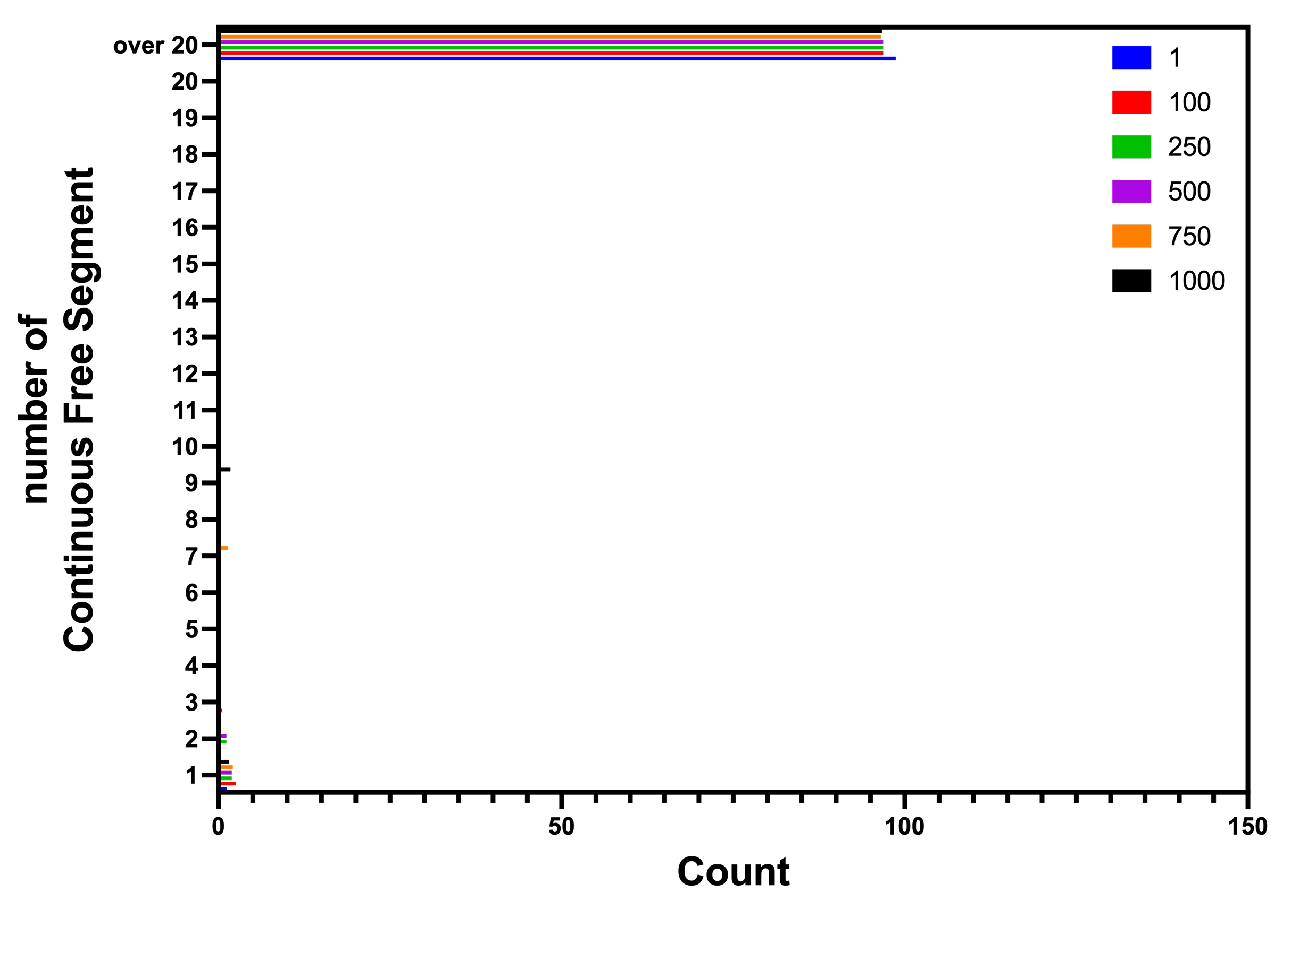
\includegraphics[width=0.95\columnwidth]{graphs/free_segment_f2fs}
	\caption{Free Segment-F2FS}
	\label{f:free_segment_f2fs}
\end{figure}

